\documentclass[10pt]{academydoc}
\pagestyle{plain}

% Set Document Details
\doctype{tb} % spec, proc, tb (Specification, Procedure, Technical Bulletin)
\docname{Informative Notes on SMPTE ST 2065-1 -- Academy Color Encoding Specification (ACES)}
\altdocname{Informative Notes on SMPTE ST 2065-1}
% Sets the document name used in header - usually an abbreviated document title
\docnumber{TB-2014-004}
\committeename{Academy Color Encoding System (ACES) Project Committee}
\versionnumber{1.0.1}
\docdate{April 24, 2015}
\summary{
This document provides notes on SMPTE Standard 2065-1 -- Academy Color Encoding Specification (ACES).
}

% Document Starts Here
\begin{document}

\maketitle

% This file contains the content for the Notices
\prelimsectionformat	% Change formatting to that of "Notices" section
\chapter{\uppercase{Notices}}
%% Modify below this line %%

\copyright\the\year{} Academy of Motion Picture Arts and Sciences (A.M.P.A.S.). All rights reserved. This document is provided to individuals and organizations for their own internal use, and may be copied or reproduced in its entirety for such use. This document may not be published, distributed, publicly displayed, or transmitted, in whole or in part, without the express written permission of the Academy.

The accuracy, completeness, adequacy, availability or currency of this document is not warranted or guaranteed. Use of information in this document is at your own risk. The Academy expressly disclaims all warranties, including the warranties of merchantability, fitness for a particular purpose and non-infringement.

Copies of this document may be obtained by contacting the Academy at councilinfo@oscars.org.

``Oscars,'' ``Academy Awards,'' and the Oscar statuette are registered trademarks, and the Oscar statuette a copyrighted property, of the Academy of Motion Picture Arts and Sciences.

% This paragraph is optional.  Comment out if you wish to remove it.
This document is distributed to interested parties for review and comment. A.M.P.A.S. reserves the right to change this document without notice, and readers are advised to check with the Council for the latest version of this document.

% This paragraph is optional.  Comment out if you wish to remove it.
The technology described in this document may be the subject of intellectual property rights (including patent, copyright, trademark or similar such rights) of A.M.P.A.S. or others. A.M.P.A.S. declares that it will not enforce any applicable intellectual property rights owned or controlled by it (other than A.M.P.A.S. trademarks) against any person or entity using the intellectual property to comply with this document.

% This paragraph is optional.  Comment out if you wish to remove it.
Attention is drawn to the possibility that some elements of the technology described in this document, or certain applications of the technology may be the subject of intellectual property rights other than those identified above. A.M.P.A.S. shall not be held responsible for identifying any or all such rights. Recipients of this document are invited to submit notification to A.M.P.A.S. of any such intellectual property of which they are aware.

\vspace{10pt}
These notices must be retained in any copies of any part of this document. \newpage
% This file contains the content for the Revision History and 
\prelimsectionformat	% Change formatting to that of "Notices" section
\chapter{Revision History}
%% Modify below this line %%

\begin{tabularx}{\linewidth}{|l|l|X|}
    \hline
    Version & Date & Description \\ \hline
    1.0     & 05/10/2013 & Initial Version      \\ \hline
    1.1     & 08/02/2013 & Modify ACESproxy to handle negative ACES values \\ \hline
    2.0     & 12/19/2014 & Modify ACESproxy primaries, constrain to legal range \\ \hline
    2.0.1   & 04/24/2015 & Formatting and typo fixes \\ \hline
            &      &             \\ \hline
\end{tabularx}

\vspace{0.25in} % <-- DO NOT REMOVE
\chapter{Related Academy Documents} % <-- DO NOT REMOVE
\begin{tabularx}{\linewidth}{|l|X|}
    \hline
    Document Name & Description \\ \hline
    S-2008-001  & Academy Color Encoding Specification (ACES) \\ \hline
    S-2014-003  & ACEScc -- A Logarithmic Encoding of ACES Data for use within Color Grading Systems \\ \hline
    S-2014-004  & ACEScg -- A Working Space for CGI Render and Compositing \\ \hline
    & \\ \hline
    & \\ \hline
\end{tabularx} \newpage

\tableofcontents \newpage

% This file contains the content for the Scope
\cleardoublepage
\numberedformat	
\chapter{Scope} 	% Do not modify section title
%% Modify below this line %%

This document specifies 10-bit and 12-bit integer encodings of ACES for use with imaging systems that produce look metadata such as ASC CDL, and with transport systems such as HD-SDI. The color encoding provided in this format represents ACES relative exposure values as RGB triplets in a logarithmic encoding, and does not define the interfaces or signals that may carry this encoding.
% This section contains the content for the References
\numberedformat
\chapter{References}
The following standards, specifications, articles, presentations, and texts are referenced in this text:
%% Modify below this line %%

Academy S-2013-001, ACESproxy -- An Integer Log Encoding of ACES Data

SMPTE ST 2065-1:2012, Academy Color Encoding Specification (ACES)

SMPTE RP 177:1993, Derivation of Basic Television Color Equations

% This file contains the content for a main section
\numberedformat
%% Modify below this line %%
\chapter{Notes on SMPTE ST 268:2014}

SMPTE ST 268:2014 -- File Format for Digital Moving Picture Exchange (DPX) is an update to SMPTE ST 268M:2003. The updated standard specifies how image data and metadata should be written to the file format when the image data is in the Academy Density Exchange Encoding (ADX). Those wishing to implement the standard should refer to the SMPTE document which can be obtained from the Society of Motion Picture and Television Engineers.
% This file contains the content for a main section
\numberedformat
%% Modify below this line %%
\chapter{Notes on Appendix A}

Those referring to S-2008-001 -- Annex B (contained in this document's Appendix \ref{appendixA}) may encounter some difficulty in trying to reproduce the tabular list of ACES RGB relative exposure values that the RICD would produce for an 18\% neutral reflecting diffuser, a perfect reflecting diffuser and a ColorChecker\textregistered chart, all illuminated by a CIE Standard Illuminant D60 source.

As written, the equations in S-2008-001 -- Annex B do not factor in the RICD camera flare that amounts to 0.5\% of the capture values of a perfect reflecting diffuser. Without the augmentation of flare, followed by the scale factor, values computed with the provided equations will be slightly off from those provided in the table.
 
Therefore, the full computation steps necessary to calculate ACES RICD relative exposure values that match those provided in the S-2008-001 Annex B table are clarified as follows:

\begin{quote}
Calculation of the values in the table listing stimulus and ACES RGB used the following elements:
	
\begin{itemize}
	\item the published CIE Standard Illuminant D60 spectral power distribution
	\item the area-normalized RICD spectral sensitivities from Annex C
	\item red, green and blue scale factors $k_r$, $k_g$ and $k_b$ which white-balance those area-normalized RICD spectral sensitivities for CIE Standard Illuminant D60
	\item hypothetical 18\% and 100\% neutral reflectors
	\item the measured reflectances of the patches on a particular ColorChecker chart
	\item camera flare amounting to 0.5\% of the capture values of a perfect reflecting diffuser	
\end{itemize}

The scale factors applied to the RICD spectral sensitivity curves are each the reciprocal of the scalar product of that curve and the illuminant. These scale factors $k_r$, $k_g$ and $k_b$ are calculated as follows:


\begin{center}
$k_r=\dfrac{1}{(I\cdot{S_r})},\quad k_g=\dfrac{1}{(I\cdot{S_g})},\quad k_b=\dfrac{1}{(I\cdot{S_b})},$	
\end{center}

where $I$ represents the illuminant and $S_r$, $S_g$ and $S_b$ represent the area-normalized spectral sensitivities from Annex C.

Once these scale factors have been determined, the ACES relative exposure values $E_r$, $E_g$ and $E_b$ are calculated as

\begin{floatequ}
\begin{gather}
E_r=S\left(\displaystyle\sum_\lambda IRS_{r_\lambda}+0.005\right), \quad\quad E_g=S\left(\displaystyle\sum_\lambda IRS_{g_\lambda}+0.005\right),\\
E_b=S\left(\displaystyle\sum_\lambda IRS_{b_\lambda}+0.005\right)
\end{gather} 
\end{floatequ}
\vspace{-20pt}

where (as before) $I$ represents the illuminant and $S_r$, $S_g$ and $S_b$ represent the area-normalized spectral sensitivities from Annex C, where $R$ represents the spectral reflectance of the object being captured, and where $S=\frac{0.18}{(0.18+0.005)}$, the flare factor from S-2008-001 4.1.1.

\end{quote}

\begin{appendices}
	\appendixchapter{Example ACESclip File XML}{i}
\label{appendixA}

\begin{lstlisting}
<?xml version="1.0" encoding="UTF-8"?>
<aces:ACESmetadata xmlns:aces="http://www.oscars.org/aces/ref/acesmetadata">
<ContainerFormatVersion>1.0</ContainerFormatVersion>
<UUID type="urn:uuid:f81d4fae-7dec-11d0-a765-00a0c91e6bf6"/>
<ModificationTime>2014-11-24T10:20:13-8:00</ModificationTime>
<aces:Info>
    <Application version="2014">Vendor_ACESmaker v3</Application>
    <Comment>Day 1 Camera A: Indoors at Area 51</Comment>
</aces:Info>
<aces:ClipID>
    <ClipName>A0001B0003FX</ClipName>
    <Source_MediaID>A0001</Source_MediaID>
    <ClipDate>2014-11-20T12:24:13-8:00</ClipDate>
</aces:ClipID>
<aces:Config>
    <ACESrelease_Version>1.0</ACESrelease_Version>
    <Timestamp>2014-11-29T23:55:13-8:00</Timestamp>
    <aces:InputTransformList status="applied">
        <aces:IDTref TransformID="IDT.Sony.Slog2.v1">
            <LinkTransform>Slog2toACES.clf</LinkTransform>
        </aces:IDTref>
        <aces:GradeRef status="preview">
            <Convert_to_WorkSpace TransformID="ACEScsc.ACES_to_ACEScc.a1"/>
            <ColorDecisionList>
                <InputDescriptor>ACEScc</InputDescriptor>
                <ASC_CDL id="cc01234" inBitDepth="16f" outBitDepth="16f">
                    <SOPNode>
                        <Description>not a real example</Description>
                        <Slope>1.0000 1.0000 0.800000</Slope>
                        <Offset>0.0000 0.0000 0.000000</Offset>
                        <Power>1.0000 1.0000 1.000000</Power>
                    </SOPNode>
                    <SatNode>
                        <Saturation>0.9</Saturation>
                    </SatNode>
                </ASC_CDL>
            </ColorDecisionList>
            <Convert_from_WorkSpace { TransformID="ACEScc_to_ACES.a1"/>
        </aces:GradeRef>
        <LinkInputTransformList>F65presetgrade_seq4.clf</LinkInputTransformList>
    </aces:InputTransformList>
    <aces:PreviewTransformList status="preview">
        <aces:LMTref TransformID="LMT.Vendor.Locon.v1.ctl">
            <LinkTransform>f34d4fae-7dec-11d0-a765-00a0c91e6bf6</LinkTransform>
        </aces:LMTref>
            <aces:RRTref TransformID="RRT.Academy.a1"/>
        <aces:ODTref TransformID="ODT.Academy.Rec709_100nits_dim.a1">
            <LinkTransform>lut1023.clf</LinkTransform>
        </aces:ODTref>
        <LinkPreviewTransformList>V1_LMTlocon.clf</LinkPreviewTransformList>
    <aces:PreviewTransformList>
</aces:Config>

<aces:TransformLibrary>
    <ProcessList id="urn:uuid:f34d4fae-7dec-11d0-a765-00a0c91e6bf6">
        <Description>Sample 3DLUT for an LMT</Description>
        <InputDescriptor>ACES</InputDescriptor>
        <OutputDescriptor>ACES</OutputDescriptor>
        <LUT3D id="lmt_prodv2" name="LMT sequence 1 day exterior" 
                interpolation="tetrahedral" inBitDepth="16f" outBitDepth="12i">
            <Description>LMT Test File</Description>
            <Array dim="33 33 33 3">
                0    0    0
                1    1    1
                [...data omitted]
            </Array>
        </LUT3D>
    </ProcessList>
</aces:TransformLibrary>
</aces:ACESmetadata>
\end{lstlisting}

	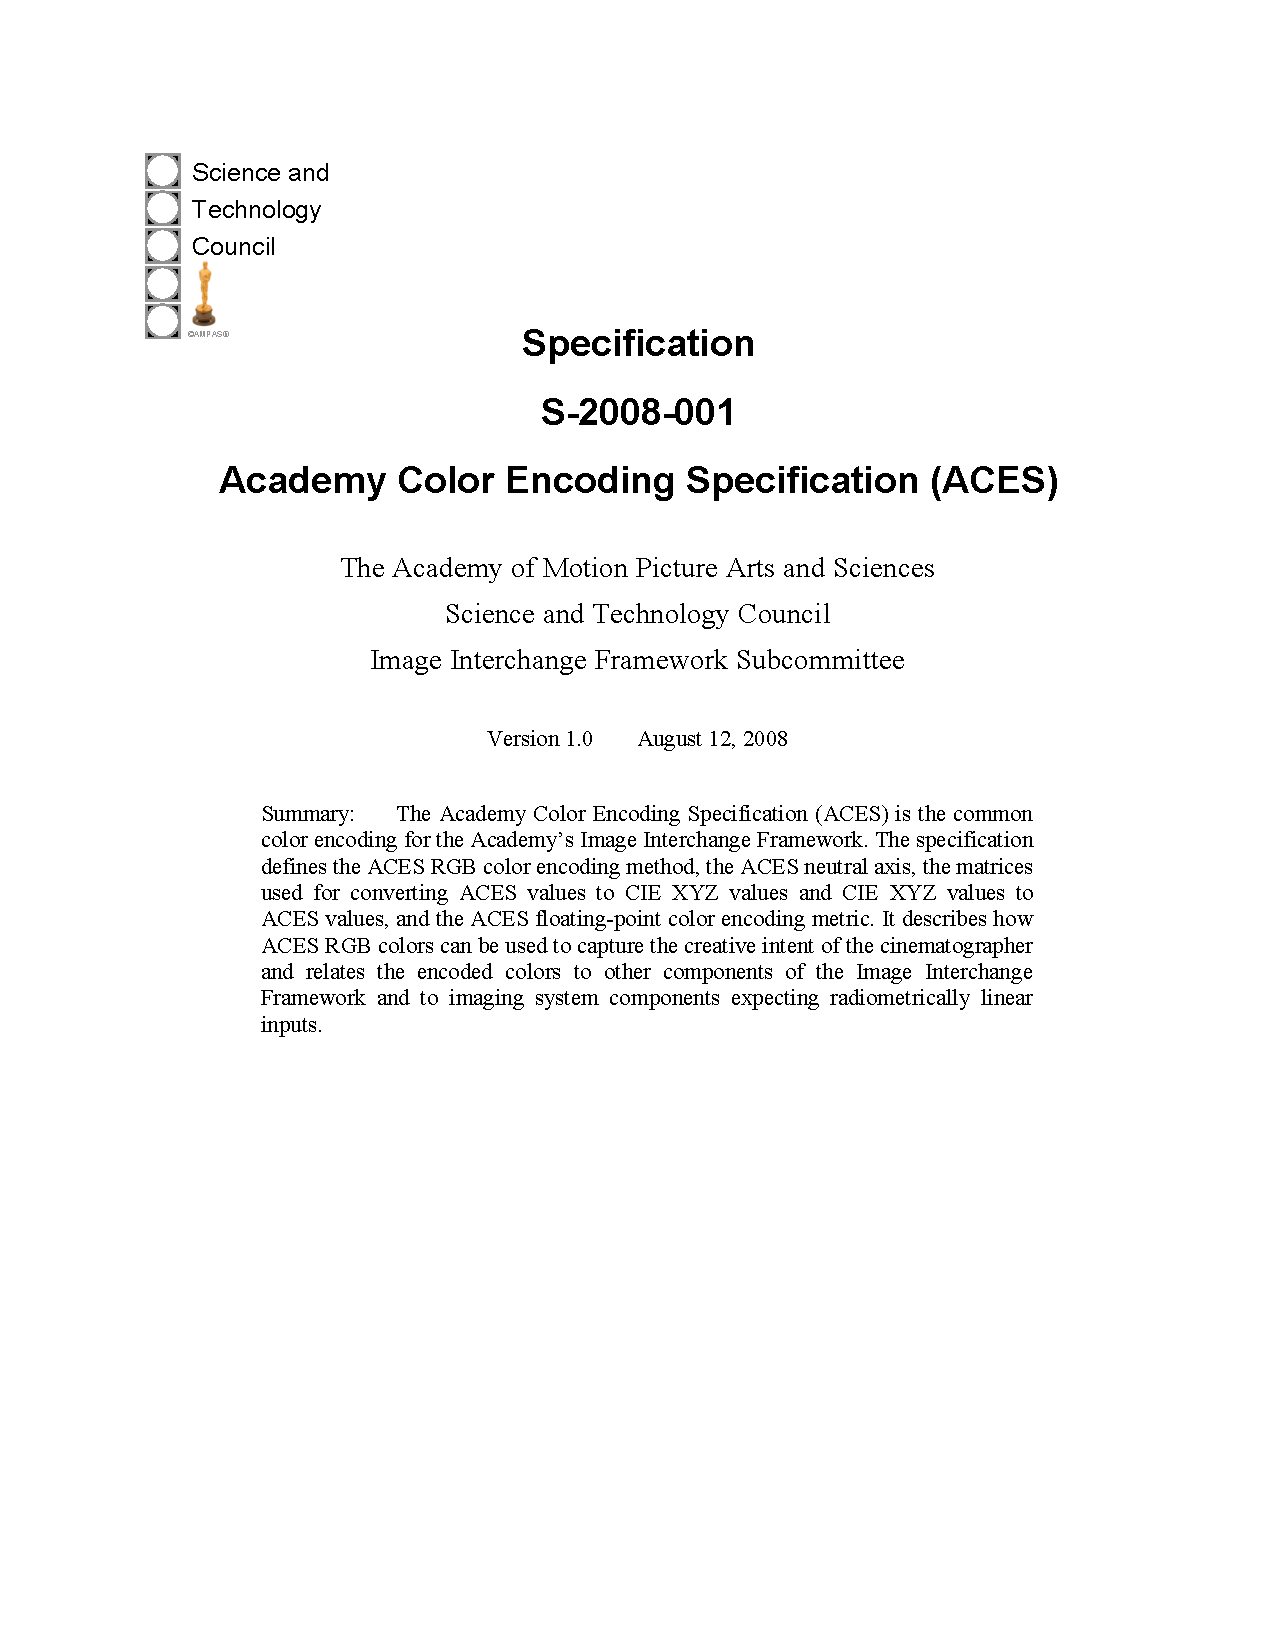
\includepdf[pages={-}]{S-2008-001.pdf}
\end{appendices}

\end{document}